\documentclass{article}
\usepackage[utf8]{inputenc}

\title{detectorhandins}
\author{Daniel S. Nielsen}
\date{October 2018}
\usepackage{siunitx} % SI units
\usepackage{cancel}  % cancel parts of equation
\usepackage{amsmath} % equations
\usepackage{tikz}
\usepackage{hyperref}

\begin{document}
	% === Front matter ====================================================

	%\frontmatter
	\maketitle
	
	\tableofcontents
	
	%\listoffigures
	
	%\listoftables
	
	%\lstlistoflistings
	
	\cleardoublepage
	
\begin{abstract}

In order to gain a better understanding of proportional gas detectors and their operation, in this experiment we describe how to build one with householding items, in particular with a cider can as the tube to be filled with gas (cathode) and a common wire from a low voltage cable (anode), and one with more advance items.
To read out the charge collected in the wire from the gas ionisation from two particle sources, Fe-55 and Am-241, the detector is connected to a preamplifier and a computer with a Multi-Channel Analyser. With the collected charge measurements we can compare the gas multiplication factor measured with the one predicted by the analysis setup and by the experimental environment. The measured values are within $1\sigma$ of the predicted values. 
A measurement of the energy spectra for Am and Fe are also possible with the experimental setup and they are usefult to identify the energy peaks for different interactions.

\end{abstract}

%\clearpage
	
	\clearpage
	\section*{Introduction}  \label{sec:Introduction}
\addcontentsline{toc}{section}{\protect\numberline{}Introduction}

	
	
	
	
	% === Main matter =====================================================
	
	% --- Chapter 1: Background -----------------------------------------------
	
	\cleardoublepage 		
	%\chapter{Theory}
	
	\clearpage
	\section{Theory}


	
	\clearpage
	\section{Experimental Setup}
\subsection{Cider can experiment}
We have been handed a start-up kit consisting of one empty $500$ ml cider can, two plexiglas endcaps, two teflon pipes, one nylon screw and nut, brass pipes and a high voltage (HV) connector with a small connector for grounding the outside of the can. \\ The process started with the preparation of the cider can which included cutting away the top part of the can, removing the inner coating with a drill with a metal brush on top, drilling a two holes in the bottom, on the the middle of the bottom part for the nylon screw and one in one side of the bottom part for the gas exchange system (of d $= 8.0$ mm and d = $6.0$ mm). The second step consisted in drilling the necessary holes in the plexiglas endcaps (which already have a groove for the can extremities to be fitted in), one hole for the gas teflon pipe in the back endcap and one in the front endcap as well as a hole for the HV connector in the front endcap (the diameters are d = $6.0$ mm and d = $9.5$ mm respectively). Finally a small hole of d = $1.0$ mm was drilled in the teflon screw, in order to fit the brass pipe in there at a later point. The brass tubes were cut and filed down with sand paper, to remove the part that was squeezed due to the cutting tool. \\ Once all the ingredients were ready, all the holes in the can and the edges of the brass tube were filed down and checked under a microscope, in order to avoid sharp edges. \\ All the components were placed in an isopropanol (IPA) bath in a sonicator, so all the skin oils and dirt were cleaned off, and the parts were dried with N$_2$ gas. At this point the only element missing was the anode wire, which was taken from a regular low voltage cable and carefully wiped with a cloth dipped in IPA. \\
The assembly of the detector commenced with the fastening of the nylon screw and bolt to the aluminium can through the hole in the middle of the bottom of the can. The longer of the two brass tubes was inserted in the nylon screw and one end of the anode wire was passed in the brass tube from the outside and pulled until the other end of the can. On the other extremity of the anode wire, a small nut was attached with a simple nod, in order to help keeping the anode wire straight later on in the process. The free end of the wire was inserted in the shorter brass tube and they were both soldered to the HV connector, which had been previously fastened to the front plexiglass endcap (and a small contact has been placed between the HV connector and the outer glass, in order to later use it for grounding the cathode). The front endcap was glued with epoxy to the cider can and was left to dry for some time. The next step consisted in straightening out the anode wire inside the can by pulling it slowly out of the can from the bottom. The wire has to be quite straight in order to avoid dips, where the charge could concentrate and ocscure the measurement. To reach an optimal condition, a weight was applied to the wire as well as careful tension. When a satisfactory straightness was achieved, the wire was soldered to the brass pipe and the rest cut off. The back endcap was glued to the cider can and left to dry for some time. \\ The gas teflon tubes were glued to the front and back endcap and a small quantity of glue was applied around the HV connector, to insure optimal insulation. \\ Before moving on to the next step, a leakage test was performed, to check for possible holes in the glue. The gas supply (in our case P$_{10}$) was attached to one of the teflon gas tubes and to a flowmeter, which measured a gas flow of approximately $25$ ml/min out of the tube. When moving the flowmeter to the other end of the can detector, the gas flow measured was between $2-4$ ml/min, which meant that an extra layer of glue had to be applied to the outside og the endcaps and to the tube connections, to cover for the leakage/leakages. After this adjustment, the gas flow was measured again and the gas flow injected in the detector was $18.3$ ml/min, while the outgoing gas flow was of $17.6$ ml/min, which was determined sufficient for the purpose of the experiment. \\ The last step consisted in removing some of the coating from the outside of the cider can with sand paper and connecting the grounding pin previously attached to the HV connector to the bare aluminuium of the can with a copper tape, to later ground the cathode to create the electric field inside the can. The connection was checked with a multimiter, where it was asserted, that there is no connection between the cathode can and the anode wire.\\
The can was attached to the P$_{10}$ gas supply with a flow of approximately $30$ ml/min for a couple of hours to remove most of the air inside for an initial test and measurement. \\ \\
Before moving on to the actual measurements, the detector was connected to the HV power supply and to the preamplifier. The output signal goes from the preamplifier to the oscilloscope through a spec. amplifier as well as from the preamplifier to the multichannel analyser (MCA) connected to a laptop, which allows data collection under the experiment. The setup was tested by feeding a few pulses with a pulse generator through the detector. During the calibration a large noise was observed due to radiations. To reduce this, an aluminium foil was used to cover the endcap and effectively shield from radiations. \\
The can detector was shortly tested with a $^{55}$Fe source to check whether a signal was visible and the test turned out to be successful. Before carrying out the actual experiment, the can detector was flushed with P$_{10}$ gas overnight.

\begin{figure}[h!]
	\centering
	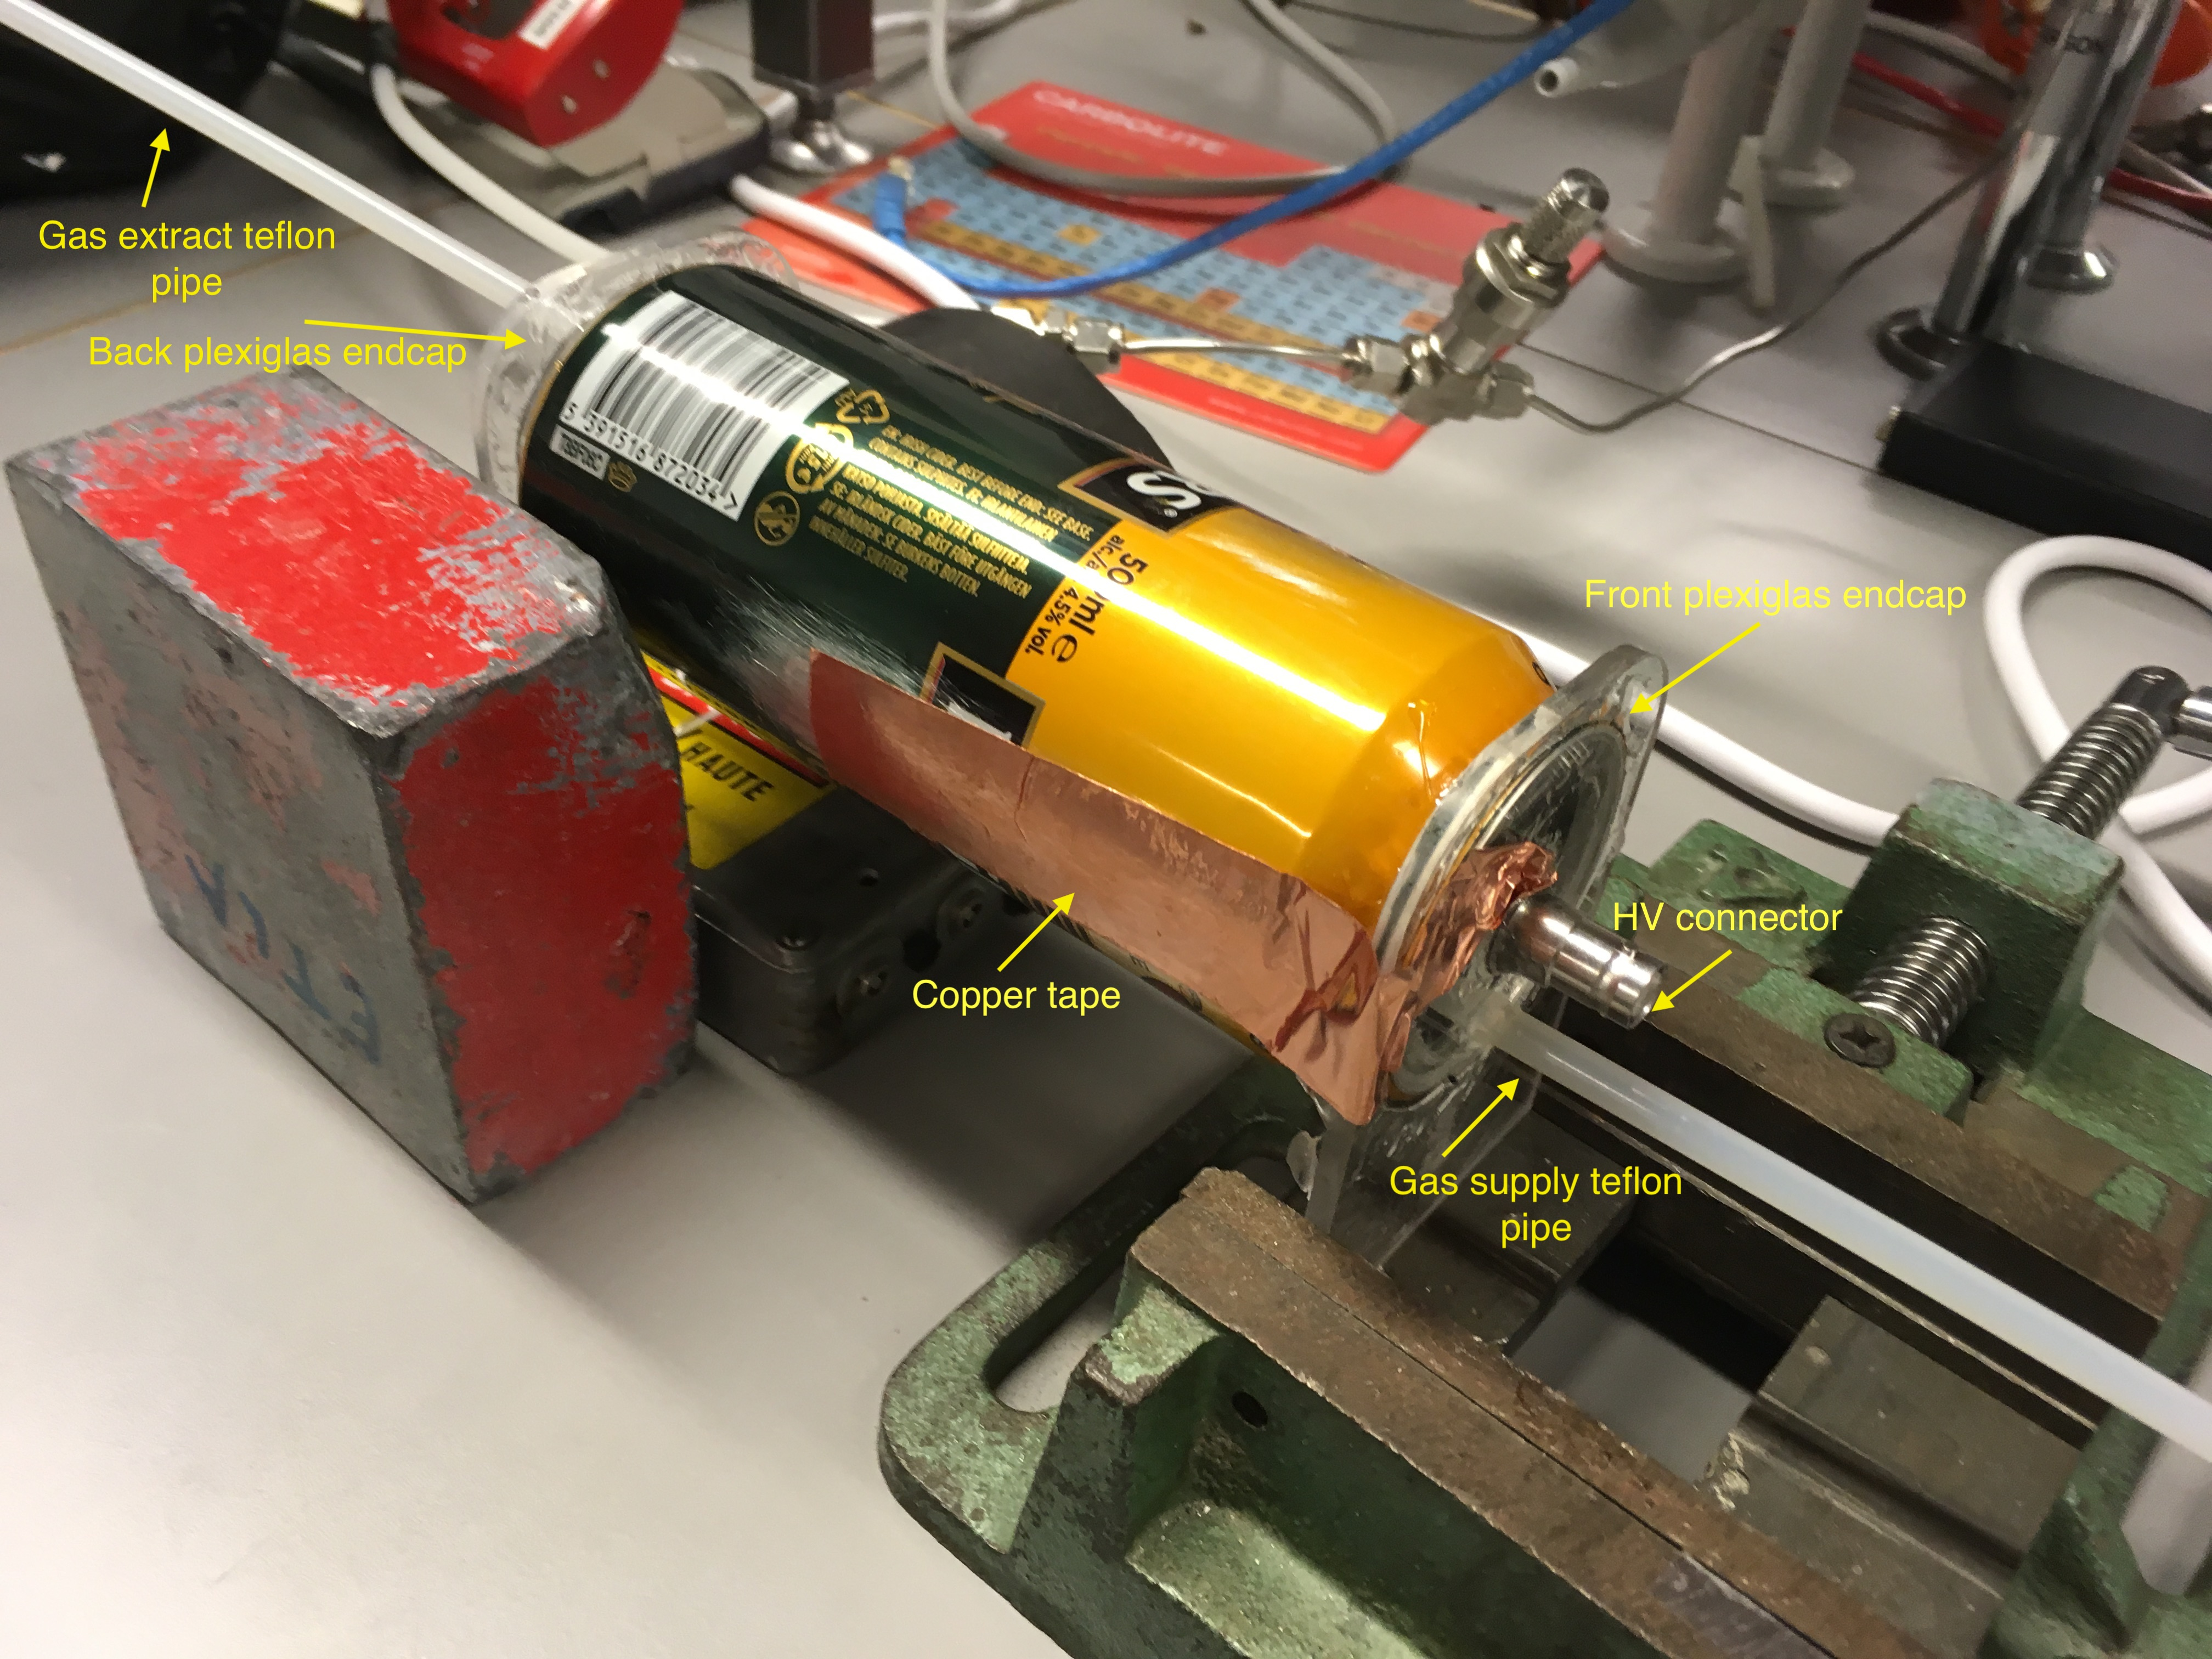
\includegraphics[width=\textwidth]{./sections/graphics/BeerCanSetup.JPG}
	\caption{Cider can proportional chamber experimental setup}
	\label{fig:BeerCan}
\end{figure}

\begin{table}[]
	\begin{tabular}{l|l|l}
			Element                  & Measurements                                          & Size                \\ \hline
			Cider can diameter       &                                                       &                     \\
			Cider can wall thickness & $105 \pm 10 \ \mu$m                                   & $105 \pm 10 \ \mu$m \\
			Plastic tube diameter    & $5.89$ mm, $5.95$ mm, $6.00$ mm, $6.01$ mm, $6.01$ mm &                     \\
			Brass tube diameter      & $1.0$ mm                                              &                     \\
			Nylon screw diameter     & $7.8$ mm, $7.75$ mm                                   &                     \\
			HV connector diameter    & $9.37$ mm                                             &                     \\
			Anode wire diameter      & $50 \pm 10 \ \mu$m                                    & $50 \pm 10 \ \mu$m 
	\end{tabular}
\caption{Measurements of the cider can experiment setup components.}
\label{Tab:cidercan_sizes}
\end{table}



\subsection{Copper pipe experiment}
For the copper pipe proportional chamber experiment we used a copper pipe, two teflon plugs, brass tubes, copper beryllium wire, teflon pipes for the gas supply, a HV connector and a grounding pin. \\
The copper pipe was filed at the edges and a hole of $5$ mm was drilled approximately in the middle of the pipe. The teflon plugs were filed down in order to match the inner radius of the copper pipe and the pre-existent holes for the gas supply tubes, HV connector and brass tube were adjusted to the appropriate sizes of the different components. The brass tubes were cut and filed following the procedure described in the previous section. All the parts were cleaned in a IPA bath and dried with N$_2$. The wire was soldered to the brass tube and to the HV connector and inserted carefully in the copper tube, avoing to cause to many curls in the wire. The copper tube was glued with epoxy to the front teflon plug. The wire was then passed into the second brass tube and in the back teflon plug  The back plug was glued and the wire solderes to the brass tube.


The measures of the different elements are noted in \ref{Tab:coppercan_sizes}


\begin{table}[]
	\begin{tabular}{l|l|l}
		& Measurements {[}mm{]}                                                  & Size \\ \hline
		Copper tube, length                        & $149.06$, $149.10$, $149.06$, $149.09$                                 &      \\
		Copper tube, wall thickness                & $1.04$, $1.00$, $1.02$, $1.02$, $1.02$, $1.14$, $1.05$, $1.04$, $1.04$ &      \\
		Copper tube, inner radius                  & $19.97$, $19.98$, $19.99$, $19.88$, $19.70$, $19.80$, $19.96$, $20.00$ &      \\
		Copper tube, radiation hole                & $5.03$, $5.04$, $5.08$                                                 &      \\
		Teflon HV front end,  total length         & $36.82$, $36.76$                                                       &      \\
		Teflon HV front end, top part length       & $15.91$, $15.94$, $15.86$                                              &      \\
		Teflon HV front end, tube extremity radius & $19.84$, $19.85$, $19.86$                                              &      \\
		Teflon back end, total length              & $15.04$, $14.97$, $14.89$, $14.93$, $14.95$, $15.06$                   &      \\
		Teflon back end, top part length           & $5.05$, $4.98$, $4.95$                                                 &      \\
		Teflon back end, tube extremity radius     & $19.88$, $19.86$                                                       &      \\
		Brass tube diameter                        & $1.0$                                                                  &      \\
		Anode wire thickened                       & $0.025$                                                                &     
	\end{tabular}
\caption{Measurements of the copper pipe experiment setup components.}
\label{Tab:coppercan_sizes}
\end{table}
	
	\clearpage
	\section{Results}
	
	\clearpage
	%\input{./sections/dicussion.tex}
	
	\clearpage
	\section{Conclusion}


	
	
	
	% === Appendices ======================================================	
	
	\appendix
	\cleardoublepage
	\section*{Appendices}
	\addcontentsline{toc}{chapter}{\protect\numberline{}Appendices}

	%\clearpage
	%\section{Resolution scans for Am and Fe}
\label{app:resolution-scans}
  \begin{figure}[htb]
  \foreach \n [count=\i] in {%
    am_100_1136,
    am_100_1191,
    am_100_1244,
    am_100_1297,
    am_100_1351,
    am_100_1399,
    am_40_1397,
    am_40_1455,
    am_40_1502,
    am_40_1559}{
   \begin{subfigure}{.5\linewidth}
        \centering
         \includegraphics[width=\linewidth]{graphics/\n}
        \caption{\detokenize\expandafter{\n}}
      \end{subfigure}
    }
  \end{figure}
  \begin{figure}[htb]\ContinuedFloat
  \foreach \n [count=\i] in {%
    am_20_1559,
    am_20_1603,
    am_20_1666,
    am_10_1665,
    am_10_1712,
    am_10_1758,
    am_4_1757,
    am_4_1808,
    am_4_1858,
    am_4_1899}{
   \begin{subfigure}{.5\linewidth}
        \centering
         \includegraphics[width=\linewidth]{graphics/\n}
        \caption{\detokenize\expandafter{\n}}
      \end{subfigure}
    }
\end{figure}
  \begin{figure}[htb]\ContinuedFloat
  \foreach \n [count=\i] in {%
    am_2_1900,
    am_2_1951,
    am_2_2001} {
   \begin{subfigure}{.5\linewidth}
        \centering
         \includegraphics[width=\linewidth]{graphics/\n}
        \caption{\detokenize\expandafter{\n}}
      \end{subfigure}
    }
    \caption{Scan for different gains and voltages for Americium.}
    \label{fig:scan:americium}
\end{figure}

  \begin{figure}[htb]
  \foreach \n [count=\i] in {%
fe_100_1420,
fe_100_1470,
fe_100_1523,
fe_100_1572,
fe_100_1617,
fe_100_1717,
fe_40_1717,
fe_40_1801,
fe_40_1853,
fe_40_1901}{
   \begin{subfigure}{.5\linewidth}
        \centering
         \includegraphics[width=\linewidth]{graphics/\n}
        \caption{\detokenize\expandafter{\n}}
      \end{subfigure}
    }
  \end{figure}
  \begin{figure}[htb]\ContinuedFloat
  \foreach \n [count=\i] in {%
fe_20_1901,
fe_20_1978,
fe_10_1978,
fe_10_2000,
fe_10_2042,
fe_10_2080,
fe_4_2080,
fe_4_2124,
fe_4_2201}{
   \begin{subfigure}{.5\linewidth}
        \centering
         \includegraphics[width=\linewidth]{graphics/\n}
        \caption{\detokenize\expandafter{\n}}
      \end{subfigure}
    }
\end{figure}
  \begin{figure}[htb]\ContinuedFloat
  \foreach \n [count=\i] in {%
fe_2_2201,
fe_2_2254,
fe_2_2303}{
   \begin{subfigure}{.5\linewidth}
        \centering
         \includegraphics[width=\linewidth]{graphics/\n}
        \caption{\detokenize\expandafter{\n}}
      \end{subfigure}
    }
    \caption{Scan for different gains and voltages for Iron.}
    \label{fig:scan:iron}
  \end{figure}

\FloatBarrier



	
	% === Back matter =====================================================
	
	% References
	%\bibliographystyle{plain}
	%\bibliographystyle{acm}
	\bibliographystyle{unsrt}
	\bibliography{./sections/references}
	\clearpage
	\pagestyle{empty}
	\cleardoublepage
\end{document}
